\documentclass{report}
\usepackage{setspace} % Setting line spacing
\usepackage{ulem} % Underline
\usepackage{caption} % Captioning figures
\usepackage{subcaption} % Subfigures
\usepackage{geometry} % Page layout
\usepackage{multicol} % Columned pages
\usepackage{array,etoolbox}
\usepackage{fancyhdr}
\usepackage{enumitem}
\usepackage[toc,page]{appendix}


%READ THIS:
%mark comments with OpenComment or ClosedComment as you write, so we can ctrl+f as needed.

% Page layout (margins, size, line spacing)
\geometry{letterpaper, left=1in, right=1in, bottom=1in, top=1in}
\setstretch{1.5}

% Headers
\pagestyle{fancy}
\lhead{PeaPod - Design Report}
\rhead{UTAG}

% Metric counter, referencing commands
% \newcounter{metricnumber}
% \setcounter{metricnumber}{1}
% \newcommand{\metricrow}{M\arabic{metricnumber}}
% \newcommand{\mlabel}[1]{\addtocounter{metricnumber}{-1}\refstepcounter{metricnumber}\label{#1}\addtocounter{metricnumber}{1}}
% \newcommand{\mref}[1]{M\ref{#1}}

\begin{document}

\begin{titlepage}
    \begin{center}
        \vspace*{1.2cm}

        \textbf{\large{PeaPod - Design Report}}

        \vspace{0.5cm}

        Primary Written Deliverable for the Deep Space Food Challenge Phase 1

        \vfill

        Jayden Lefebvre - Lead Engineer\\\small{jayden.lefebvre@mail.utoronto.ca}\\
        \vspace{1cm}
        Nathan Chareunsouk, Navin Vanderwert, Jonas Marshall - Design Engineers

        \vspace{2.5cm}

        Revision 0.2\\
        University of Toronto Agritech\\
        July 1st, 2021

    \end{center}
\end{titlepage}

\thispagestyle{plain}

\tableofcontents
\newpage

\section{Design Abstract}
% Please provide a brief summary description of your proposed food production technology within a 1,500 character limit. The abstract may answer some of the following questions: What is your proposed solution? What is novel, sustainable, and innovative about your proposed solution? What types of food does your solution create? How are you minimizing inputs and maximizing food outputs?
Our solution is a modular aeroponic plant growth environment based upon controlled-environment agriculture principles.
The ability to precisely control environmental parameters allows our system to grow any plant imaginable.

\section{Design Report}

\subsection{Description}

\textbf{Part A}

% ===== PROMPT =====

% Please provide a more fulsome description of your food production technology. Your description needs to include information about what the technology is, what it does, how it functions, and how the crew will interact with it. Be sure to also provide any descriptions of major hardware components and processes in relation to your technology.

% ===== WRITE =====
% 3000chars

% Your response should include the following:

% Environmental Control Parameters
    % Nutrient Solution (pH, Watering Cycle, Plant Nutrient Dosages)
    % Leaf- and root-zone temperatures
    % Leaf-zone humidity
    % Lighting intensity, spectrum, cycle
% Outputs
    % Plant Mass, O2, Waste
% Data Collection
    % Environment Parameter Collection
    % Plant Metrics
        % Post-harvest analysis (harvest weight/wt.\%, chemical composition i.e. nutrients, flavour)
        % Live Mass/Growth Rate
        % Visual analysis via computer vision (canopy surface area, leaf health indicators, number of leaves, plant height, etc.)
% Crew Interaction
    % Planting
    % Manual inputs (nutrient and water reservoir refill)
    % Setup (Assembly, hookup to peripheral systems)
    % Harvest?

An automated and isolated aeroponic crop growth system, able to generate any environment from a combination of independent environment parameters, with both environment and crop growth data collection.
The system takes the form of an enclosed cube, with most crew interaction limited to water and nutrient refill. Hardware components can be broken down into 4 primary categories: Feedback Systems, Resource Supply, Support Structures, and Electronic Control. 
Together, these 4 components create the "Black Box" seen in Figure \ref{fig:blackbox}.

\begin{figure}[h]
    \centering
    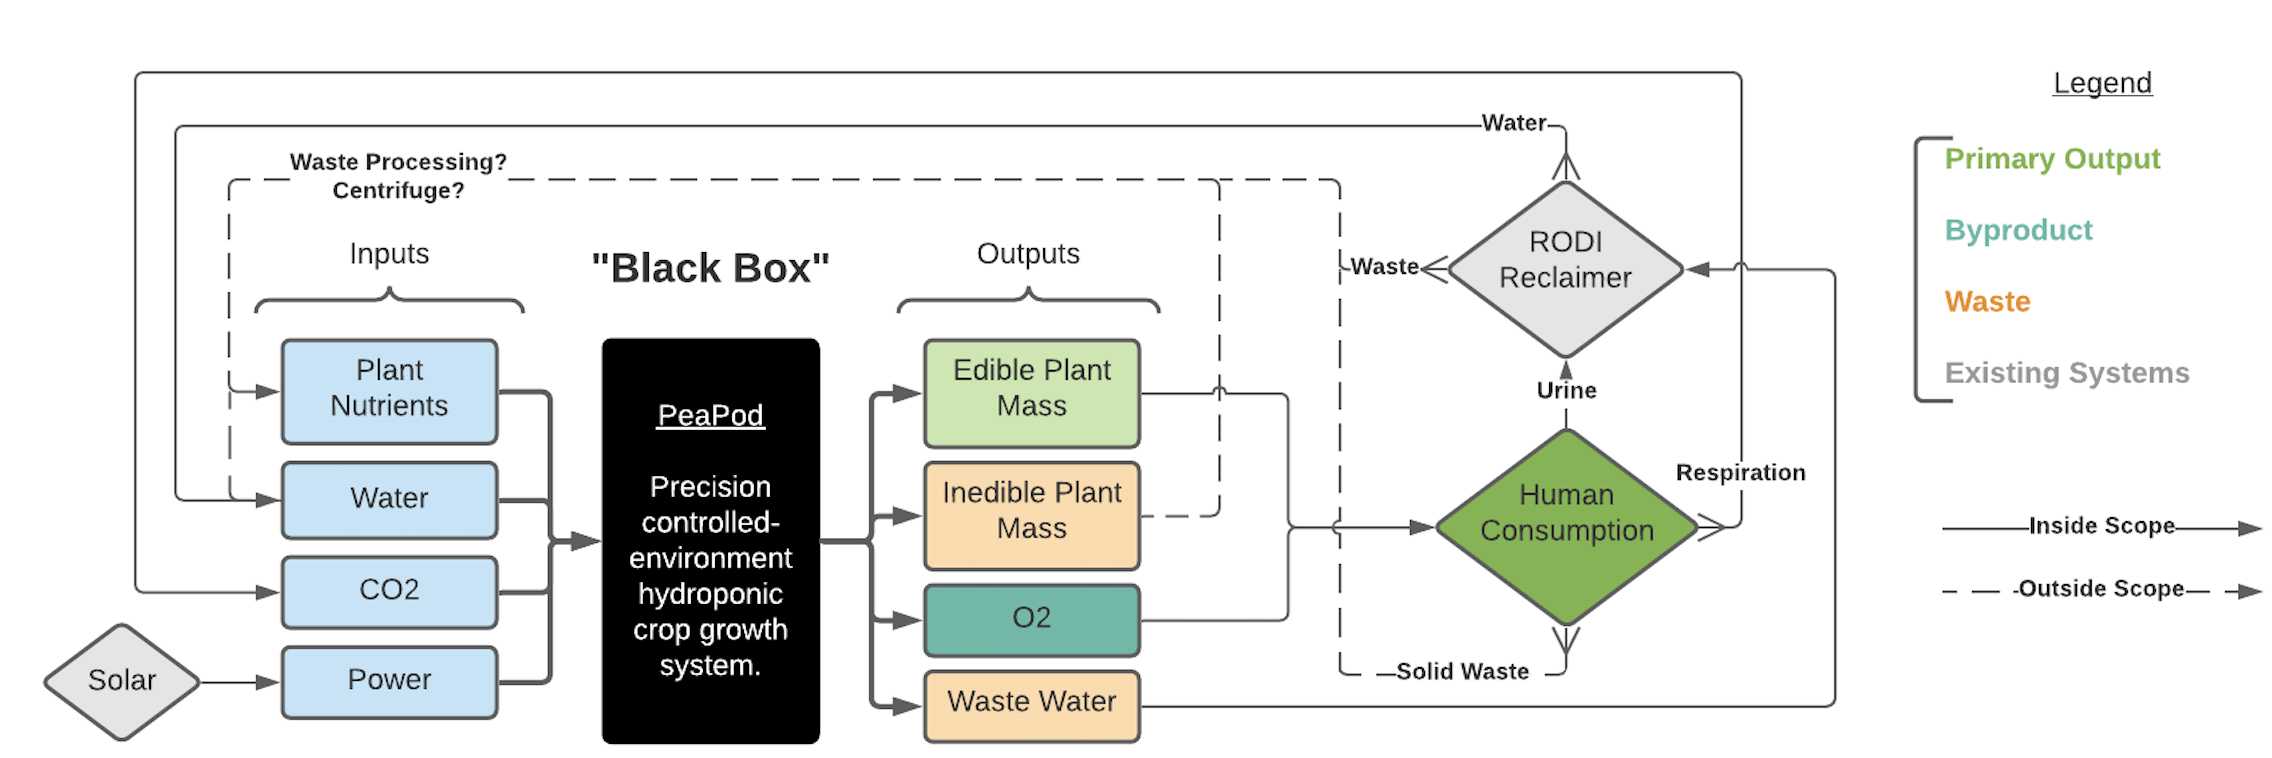
\includegraphics[width=15cm]{../solutionoverview/images/blackbox.png}
    \hfill
    \caption{"Black box" function diagram for our solution.}
    \label{fig:blackbox}
\end{figure}

\textbf{Part B:}

% ===== PROMPT =====

% Please describe the basic operations concept of the food production technology. In your response, describe assumptions required of operation. You can also include, for example, details about whether a sterile/aseptic environment is needed, if special steps are required between production cycles, or if fluids or materials must be removed or added to prime/inoculate a system.

% ===== WRITE =====
% 1500chars

% Setup
    % Prime plant inputs (connect power/water supply, prime aeroponic pump/tank/etc.)
    % Set parameters (set manually or to a preset e.g. “Spinach”)
% Operation is then automatic, with PeaPod regulating conditions and notifying the user if maintenance is required
% Maintenance can include:
    % Replenishing water and nutrient stores
    % Replacing/repairing failed components
    % Observation
    % Cleaning the aeroponic nozzle
% Collection is removing the plant from the enclosure
% Priming for next cycle is dependent on required maintenance as informed by PeaPod

\subsection{Innovation}

% ===== PROMPT =====

% This question seeks to establish an understanding of how your technology is different from other technologies that currently exist. Your description needs to be clear and well defined using simple language when detailing how your food production technology is novel, innovative and sustainable. Ensure to provide examples that will portray the novelty of your technology. 

% ===== WRITE =====

% Elaborate on these:
% Wide, continuous, precise control
% Environment optimization for output metrics

\subsection{Adherence to Constraints}
% ===== PROMPT =====

% Whether in space or in a remote community on Earth, there are several constraints that your food production technology should adhere to. This question outlines key constraints below that your technology will need to address.

% NOTE: In Phase 1, Adherence to Constraints is not meant to determine whether the Design Report itself is complete in including all the required information. This question is meant to ensure that Teams have considered the constraints, and that the food production technology design, at a minimum, falls within those constraints. In future Phases, Teams’ food production technologies will be evaluated and scored on whether or not the design stays within the constraints so that it ultimately can meet CSA’s needs and deliver value.

\subsubsection{Outer Dimensions, Volume} 

%Fits through 1.07m x 1.90m doorway; W < 1.820m, D < 2.438m, H < 2.591m; V<= 2m^3

% How did we consider this constraint in the formulation of our design? Our feature/component/subsystem selection? Does it fall wihtin the proposed constraint?

% 300chars

\subsubsection{Power Consumption} 

%Avg <1500 W, Peak < 3000 W

% How did we consider this constraint in the formulation of our design? Our feature/component/subsystem selection? Does it fall wihtin the proposed constraint?

% 300chars

\subsubsection{Water Consumption}

% ===== PROMPT =====

% Unconstrained

% How did we consider this constraint in the formulation of our design? Our feature/component/subsystem selection?

% ===== WRITE =====
% 300chars

\subsubsection{Mass} 
% ===== PROMPT =====

%Unconstrained

% How did we consider this constraint in the formulation of our design? Our feature/component/subsystem selection?

% ===== WRITE =====
% 300chars

\subsubsection{Data Connection} 
% ===== PROMPT =====

%Unconstrained

% How did we consider this constraint in the formulation of our design? Our feature/component/subsystem selection?

% ===== WRITE =====
% 300chars

\subsubsection{Crew Time Requirement - Setup \& Maintenance} 
% ===== PROMPT =====

%4 hrs/week

% How did we consider this constraint in the formulation of our design? Our feature/component/subsystem selection? Does it fall wihtin the proposed constraint?

% ===== WRITE =====
% 300chars

\subsubsection{Palatability of Crop Output} 
% ===== PROMPT =====

%>= 6.0 Hedonic

% How did we consider this constraint in the formulation of our design? Our feature/component/subsystem selection? Does it fall wihtin the proposed constraint?

% ===== WRITE =====
% 300chars

Hydroponic crops have seen commercial success, suggesting that their output is of sufficient hedonic quality to be desired. Additionally, PeaPod is designed to optimize for edible plant mass, nutrient denisty, and other health indicators---pushing hedonic quality up over time.

\subsubsection{Operational Constraints} 
% ===== PROMPT =====
% Terrestrial (see requirements)

% How did we consider this constraint in the formulation of our design? Our feature/component/subsystem selection? Does it fall wihtin the proposed constraint?

% ===== WRITE =====
% 300chars
 
\subsection{Performance Criteria}

% NOTE: This section seeks to understand how the proposed food production technology addresses the performance criteria of the Challenge. Describe how the food production technology addresses the following performance criteria.

\subsubsection{Acceptability}

\textbf{Acceptability of Process}
% ===== PROMPT ===== 
% Describe in detail the processes and procedures of using your technology.
% Please also provide an assessment (using industry standards and/or existing research) that your technology processes are likely to be user friendly and acceptable to the crew.

% Target: The process must be something crew members could be expected to accomplish in a reasonable amount of time, on a daily basis in a small kitchen-like space after a busy workday.
% Teams should consider the current target for Astronauts is 1 hour per meal (30 minutes for preparation, 30 minutes for the meal itself). 

% ===== WRITE =====
% 3000chars

% Include each of the following:
    % Operational footprint (how much space is needed for the solution and its related processes?)
    % Setup steps
    % Food production cycle
    % Food handling 
    % Cleaning and stowage procedures of equipment
    % Time needed for the crew to operate the solution

\textbf{Acceptability of Food Products}

% ===== PROMPT =====
% Please provide an assessment (using industry standards and existing research) that the food outputs of your technology are likely to meet the acceptability target. 
% Rate and describe the potential acceptability of your food products on a 9 point hedonic scale. The hedonic scale is a quantitative method that is accepted throughout the food science industry as a means to determine acceptability. 
% Further information regarding methods for determining food acceptability can be found in references such as Meilgaard, Morten C., B. Thomas Carr, and Gail Vance Civille. Sensory evaluation techniques. CRC press, 2006.

% Target: A food item measuring an overall acceptability rating of 6.0 or better on a 9-point hedonic scale for the duration of the mission is considered acceptable. 

% ===== WRITE =====
% 3000chars
% NOTE: You should be as descriptive as possible in your response. 

% Include:
    % Appearance
    % Aroma
    % Palatability
    % Flavor
    % Texture

% Optional - Additional comments
% This additional text box with a 1,000 character limit allows you to provide any other information on acceptability and palatability you would like to submit to the Judging Panel.

\subsubsection{Safety}

% The overall safety of the food production process and the food products are a top priority for this Challenge.
% NOTE: No pathogens are permitted to exist within the food technology or its outputs.  Teams must take this into account in their Phase 1 designs. Designs that fail to account for pathogens will receive a "fail" score on the Safety category.

\textbf{Safety of Process}

% ===== PROMPT =====

% Your answer will need to describe the safety associated with the food production process using your technology. The food production process includes: the safety of the food handling or processing procedures and environmental safety. Please include all food safety procedures that need to be followed.

% Targets:
    % Avoidance of hazardous compounds or materials used or produced (e.g., microbes, off-gassing, toxic components) 
    % Avoidance of hazards associated with cleaning this technology prior to and/or after use
    % Avoidance of physical, chemical, or biological hazards associated with the hardware or the process
    % No pathogens (i.e. nitrogen fixing bacteria); all nutrients provided directly
    % Clear mitigation strategies to address the aforementioned risks

% ===== WRITE =====
% 3000chars

% Include risk assessment/understanding, as well as mitigation, for both production and output handling processes.

\textbf{Safety of Food Products}

% ===== PROMPT =====
% Your answer will need to describe the safety of the resulting food products (outputs), including safety for repeated human consumption.

% Target: Consumption safety: Resulting food product is safe for repeated human consumption as defined by NASA-STD-3001 (see Reference Materials)

% ===== WRITE =====
% 3000chars

% Optional - Additional comments
% This additional text box with a 1,000 character limit allows you to provide any other information on the safety associated with the food production process using your technology.

\subsubsection{Resource Inputs and Outputs}

% NOTE: In your response, you will need to describe the resource requirements of the food production process (inputs) and all outputs. You will need to also include the estimated quantities of each input and output, as well as the nutritional quality of the food product.

\textbf{Resource Inputs}

% ===== PROMPT =====

% Indicate the inputs needed to run your food production technology
% Inputs may include: Raw materials, energy, water, or other materials that enter the system.

% ===== WRITE =====
% 3000chars

% Describe resources, and their quantities

\textbf{System Outputs}

% ===== PROMPT =====

% Indicate the outputs generated from your food production technology. 

% ===== WRITE =====
% 3000chars

% Include: 
    % Food products
    % Waste
    % Heat (latent and sensible)
    % All other usable or unusable products exiting the system, including liquid and gaseous process flows (e.g., water vapor, low-molecular weight organic and inorganic compounds, water, oils, etc.).

\textbf{Optimization}

% Provide a description on how the food production technology achieves the greatest amount of food output in relation to the quantity of inputs and quantity of waste output. 

% Maximum quantity food output relative to quantity of system inputs
% Maximum quantity food output relative to quantity of waste output

% ===== WRITE =====
% 1500chars

Maximizing output is perhaps the greatest strength of PeaPod. Since it is fully automated, growth cycles have a high degree of certainty that let researches hone in on the perfect conditions---and then repeat them ad infinitum.
By collecting data in an isolated environment like this, optimization can be done on any number of parameters, including quantity of inputs. As trials are conducted and PeaPod gathers data, it measures the quantity of inputs taken and a plethora of plant data related to usable quantity, bringing PeaPod to the most efficient conditions over time.
In addition, the array of sensors used to collect data double as input for PID control, letting PeaPod react to unpredictable events such as poor seed health and salvage otherwise poor outputs.

\textbf{Food Output Quality}

% ===== PROMPT =====

% Please describe  the nutritional quality of the resulting food products from your technology. You will need to provide the nutritional potential of the food produced with your technology. Use values based on reasonable literature information that you can reference. For example, as defined by NASA-STD-3001 (see Reference Materials).

% Targets:
    % Maximum macronutrients supplied, as a percentage of a crewmember’s complete dietary needs
    % Maximum micronutrients supplied, as a percentage of a crewmember’s complete dietary needs
    % Maximum variety of nutrients supplied

% ===== WRITE =====
% 3000chars

% Optional - Additional comments
% This additional text box with a 1,000 character limit allows you to provide any additional information on the resource inputs and outputs related to the use of the food production technology.

\subsubsection{Reliability and/or Stability}

\textbf{Process Reliability}

% ===== PROMPT =====

% Please provide a description of the reliability of your technology.

% Target: Less than 10\% loss of functionality or food production throughout a three-year mission.

% ===== WRITE =====
% 3000chars

% Include:
    % Operational lifespan
    % Percentage of functionality lost over 3 years
    % Maintenance process, procedures, schedule, incl. component maintenance/replacement and spare part requirement

%OpenComment pretty barebones, might need citations for material duration... feel free to add anything else that sells the reliability - NV
By nature of its design, PeaPod will last three years at near 100\% functionality on minimal maintenance.
This is achieved by self-monitoring component health, using servicable materials, and providing smart notifications to the user when maintenance is needed.
For one, PeaPod is designed to be assembled by a single user with readily available tools. This means it can be disassembled, cleaned, and put back together by one person in a non-restrictive amount of time.
For another, the sensors used to monitor plant health and growing conditions allow PeaPod to notify the user when a part needs to be fixed or replaced. For example, if humidity readings fall below historical levels for current water output, PeaPod will notify the user to replace the insulating material in the nozzle area. If light intensity begins to drop in a certain sector, PeaPod will tell the user to replace a certain bulb.

This said, every component in PeaPod has an expected lifespan over three years. From the LEDs (rated for 5 years) to the nozzle (only needs periodic cleaning) to the bonding agents (tested for materials used), replacement monitoring is only needed as a backup.

Scheduled maintenance breaks down to three primary tasks: refilling nutrients, cleaning spray nozzle, and harvesting/replacing plants.
Since PeaPod mixes the nutrient solution automatically, the only required maintenance is replenshing stores of water and individual nutrients. By tracking consumption rates and using past trends, PeaPod can schedule the most efficient refill time in advance and notify the user.
The spray nozzle, by way of its fine mesh, will build fine amounts of sediment over time. This can be easily cleaned by the user at either pre-determined times or, as mentioned above, when the unit detects an issue.
Finally, plant harvesting is a quick task that simply constitues opening the unit and removing the plant. Replacing it only requires the user to open the unit, place the seed in the grow cup, and digitally set the grow conditions for PeaPod to follow.

\textbf{Input and Output Stability}

% ===== PROMPT =====

% Provide a description of the stability of both the input products used and food product outputs.

% Target: Longest possible shelf-life of the input and food products. They must remain safe, without any significant loss of nutritional value or quality at ambient conditions

% ===== WRITE =====
% 1500chars

% Include:
    % Inputs shelf life
    % Outputs shelf life
    % Reasoning for the above
    % Degree of loss of quality (i.e. shelf life deterioration)

PeaPod's input stability is maximized by a variety of design choices, the sum of which give them a shelf life above the three-year mark of a mission. Since the system doses nutrients automatically and at a high-degree of precision, nutrient solution can be stored at a much greater density than would be possible with manual mixing. This minimizes degradation and loss of quality while reducing the space needed to store the solutions. Since the solutions can be stored in such a compact manner, it is feasible to store them in an insulated, opaque container that minimizes fluctuations in environment that could stimulate degredation. And, by utilizing the electrical infrastructure of PeaPod itself, it is trivial to maintain a set temperature within this container that further hampers deterioration.

Outputs will have a shelf life that is, in worst case, comparable to fresh produce grown outdoors. More realistically, crops are expected to last longer as a result of a lack of pests, disease, and optimization of characteristics for ambient conditions nearby. These are the result of PeaPod's isolated enivornment and data collection capabilities. For example, the same sensors used to optimize growth conditions can then be used to optimze traits for the given storage conditions, letting researchers select for crops and characteristics that will last the longest. Finally, PeaPod can let users grow crops on a rotation, providing a steady supply of fresh produce that will not need to be stored for particularly long periods of time, thus circumventing some of the restrictions posed by growing fresh crops.

% Optional - Additional comments
% This additional text box with a 1,000 character limit allows you to provide any other information on reliability and stability you would like to submit to the Judging Panel.

\subsection{Terrestrial Potential}

% ===== PROMPT =====

% Describe your vision of your food production technology’s potential to improve food production on Earth. Provide a concrete scenario in which your technology would serve the community in which it operates.

% ===== WRITE =====
% 3000chars

\textbf{Customer-facing Food Service} %OpenComment does this make sense? feels a little weak/unfounded - NV

At present, a restaurant requires either a local supplier or a substantial amount of outdoor space (and labour) to serve fresh produce. Both of these are cost-prohibitive, and the latter is entirely impossible in many situations. Local suppliers' high costs are the result of a few things:
\begin{itemize}
    \item Limited seasonal availability
    \item Frequent transport need
    \item High costs with little demand
\end{itemize}
PeaPod has the potential to reduce these barriers in a cyclic way. Partnerships between local suppliers and restaurants will provide these restuarants with space- and time-efficient PeaPod units with the purpose of generating both produce and data. The increase in produce will reduce the frequency at which suppliers need to make deliveries, while the data produced will let suppliers maximize output. Over time, this can increase efficiency to the point where local suppliers can provide produce at a lower price.

\textbf{Crowdsourced Research} %ClosedComment feel better about this one, almost like a better version of the above ^ - NV

Due to PeaPod's automated nature, off-site research is a feasibile method of collecting data. As a result, universities and other institutions can save costs related to space and energy usage by subsidizing PeaPods to consumers, schools, or even restaurants. Users would receive sets of paramters within which to grow crops, and the data would be sent back to the institution. The user can use the produce, at the cost of space and energy, while the institution continues to provide parameters with which to grow. The end result is a massive set of data, conducted in identical conditions in different places, verified by comparison with the myriad devices conducting the same tests.

\textbf{De-centralized Production} %ClosedComment I like this one, should add more though - NV

Many crops are only feasible in certain climates, making global transport a necessity to sell them worldwide. This reduces freshness, necessitates various preservatives, and increases carbon consumption. By upscaling PeaPod technology to a farm scale, it becomes possible to produce climate-bound crops in any location. This creates region-based farms that can produce a tremendous variety of crops, vastly reducing transport needs and making it easier to have a local food diet.


% Q2.6. Supporting Material 
% Q2.6.1. Include any visual representations of the food production technology, which may include models, schematics, or drawings.
% You are required to submit (a) visual representation(s) of your proposed technology. You should submit these visuals in a document in PDF format, of maximum five (5) Letter Size pages (8.5” x 11”).
% Q.2.6.2. Optional: Include any preliminary data or calculations that support the design and operation of the food production technology.
% You may submit a document in PDF format, of maximum two (2) Letter Size pages (8.5” x 11”), including preliminary data or calculations. 

% \newpage

% References
% \bibliographystyle{IEEEtran}
% \bibliography{references}
\end{document}